%%%%%%%%%%%%%%%%%%%%%%%%%%%%%%%%

\section{Near Detector Prototypes}
\label{sec:proto-nd}
Near detector prototypes are planned for both the neutrino detector and beamline measurements systems.

\subsection{Near Neutrino Detector Prototypes}
\label{sec:proto-nd-nnd}
The prototyping plan for the Fine-Grained Tracker (FGT) near neutrino
detector, as described in Section~\ref{cdrsec:detectors-nd-ref},
involves the following major steps:
\begin{itemize}
\item Straw-Tube Tracking Detector (STT) Prototyping
\item ECAL Prototyping
\item MuID -- RPC Development
\item Dipole Magnet Studies
\end{itemize}

A schematic of the FGT is given in
Figure~\ref{fig:STT_schematic}. The prototyping activity for the
reference design %, as proposed in the CDR, would 
is proposed to be taken up jointly by
the participating collaborators in India, with some contributions from institutions in
the U.S. or other countries. %possible institutions.  
The prototyping work is spread
over a duration of three years. The %present 
ongoing efforts in this
direction are detailed below.

\subsubsection{Straw-Tube Tracking Detector}

The proposed Straw-Tube Tracking (STT) detector design
provides the central active tracking of the FGT and use straws of
1-cm diameter fabricated from an inner carbon-loaded Kapton (XC) wall
and a second aluminum-coated outer Kapton (HN) wall. The details of the
STT are available in
Section~\ref{cdrsec:detectors-nd-ref-fgt-stt}. The prototype design
has two layers of 60 straws each.  The straws used will have the
same dimensions as listed in
Section~\ref{cdrsec:detectors-nd-ref-fgt-stt}, but half the nominal
length, i.e., 1.8~m. The major milestones in the STT prototyping
(during the initial three years) are highlighted below.

%\textbf{\textit{Design and Fabrication of STT Prototype}} \\
The three-year STT R\&D and prototyping phase will start with the 3D
design of a prototype module.  This will include optimizing
parameters from the prototype assembly point of view and
establishing its mechanical structure and strength using the Finite Element Method (FEM) 
techniques. This process will be a self-feeding system with inputs
also from the GEANT detector simulations.
Figure~\ref{fig:STT_SimulationG4} shows some of the ongoing work. 
%We plan to fabricate t
The STT prototype will be fabricated and  will undergo %to perform
extensive tests both in the laboratory and %by exposing it to 
in particle
beams at CERN.

\begin{cdrfigure}[Basic GEANT4 Simulations of 1-cm straws for the prototype plan]
{STT_SimulationG4}{Basic GEANT4 Simulations of 1~cm straws for the prototype plan}
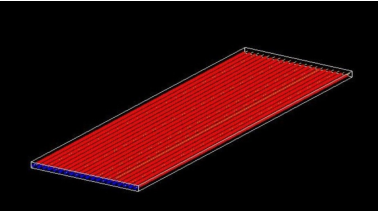
\includegraphics[width=0.6\textwidth]{STT_SimulationG4}
\end{cdrfigure}


%\textbf{ \textit{Design and prototyping of radiators and nuclear targets}} \\
As described in Section~\ref{cdrsec:detectors-nd-ref-fgt-stt}, a key
feature of the STT is the capability to integrate a series of
different nuclear targets for (anti)neutrino interactions.  The main
target is provided by the radiators that are made of thin polypropylene foils
(Figure~\ref{fig:STT_Detail}).  The design of the radiator targets has
been optimized with simulations of the Transition Radiation (TR) and
with emphasis on their integration into the mechanical structure of
the STT modules.  The production and design of the plastic foils was
discussed with vendors and %we plan 
it is planned to produce a half-scale
(1.8~m$\times$1.8~m) prototype of the radiator targets to demonstrate
the assembly, the mechanical properties and the overall
performance as well as to
further optimize the design of the tubes, including the tube diameter
and the possibility to use C-composite tubes. 
A preliminary design has been developed for the
pressurized Ar gas target (Figure~\ref{fig:STT_ArTargets}), based on
the use of 0.5-in diameter aluminum tubes.
\begin{cdrfigure}[Design of the target plane with pressurized Ar gas]
{STT_ArTargets}{Design of the target plane with pressurized Ar gas.}
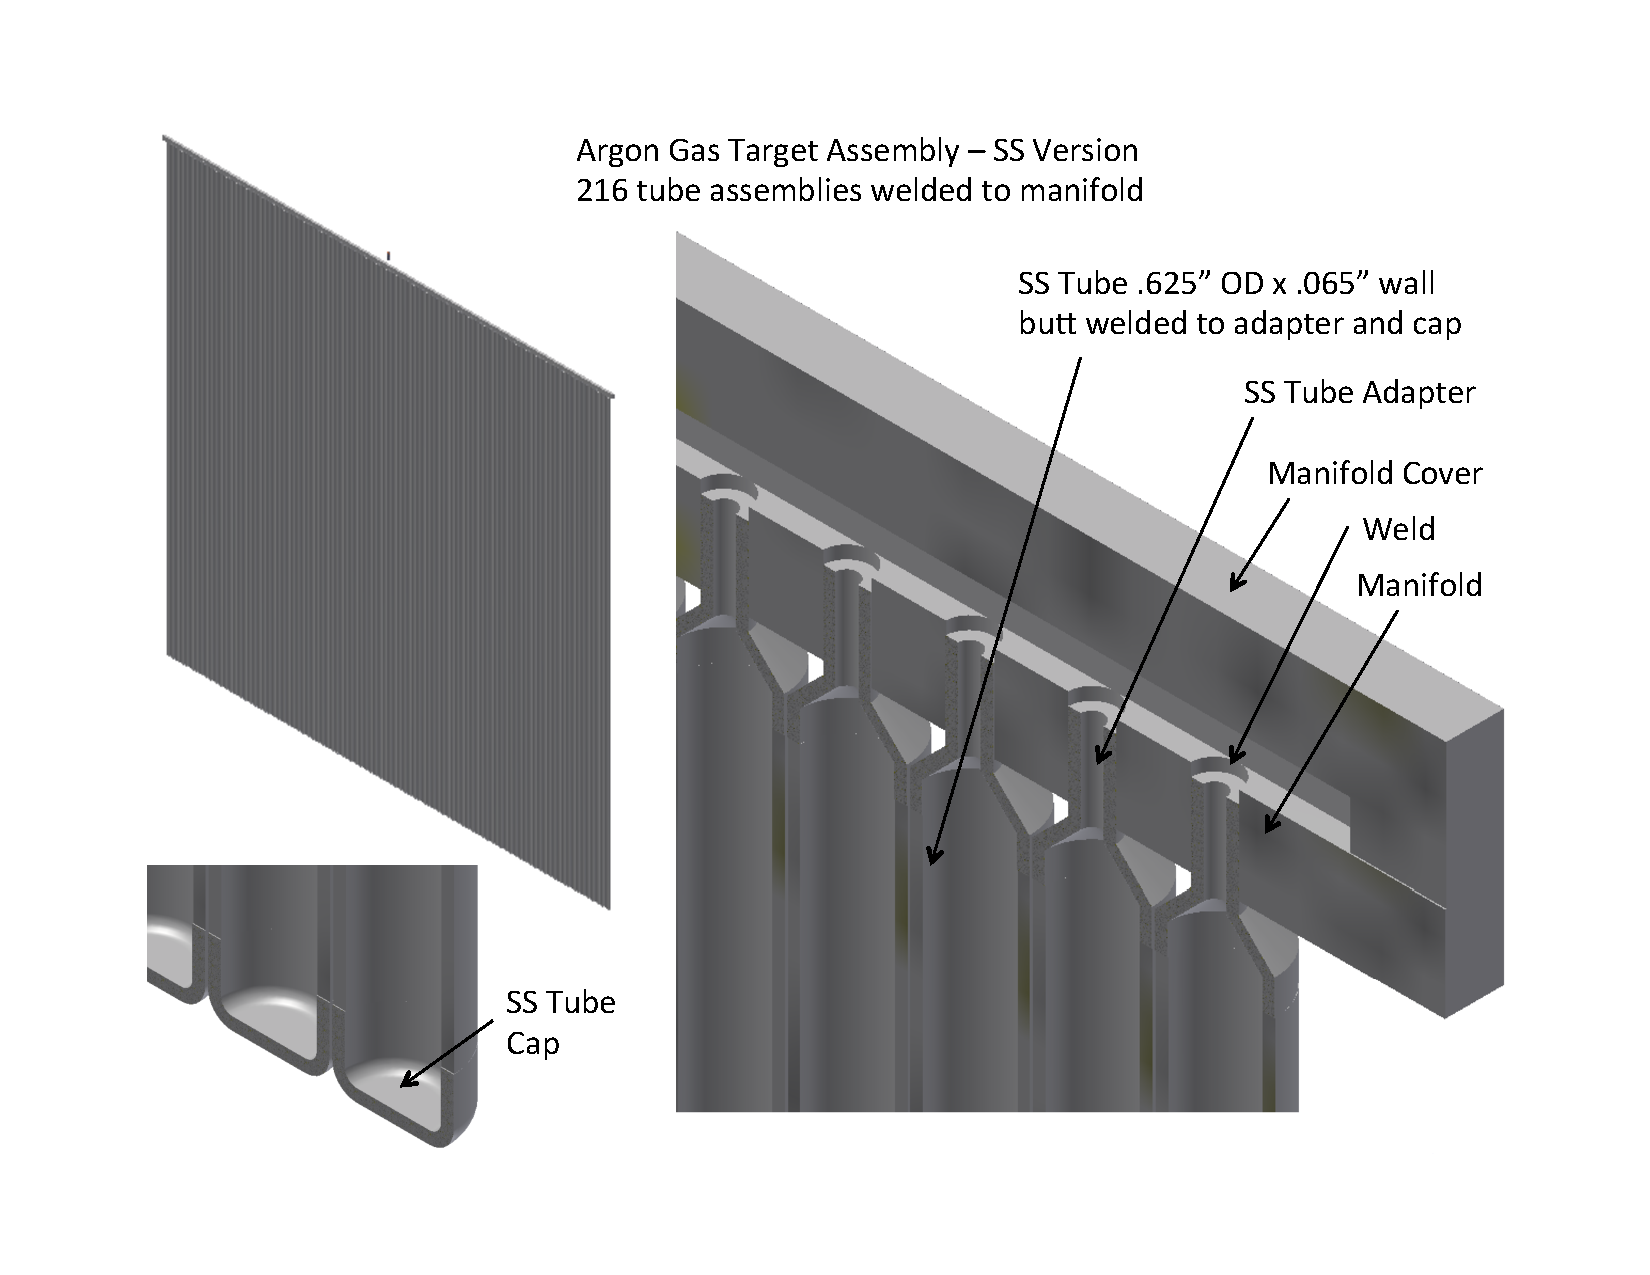
\includegraphics[width=0.6\textwidth]{STT_ArTargets}
\end{cdrfigure}

Construction of small-scale prototypes of the Ca and C targets is also planned.


%\textbf{ \textit{Anode Wire Studies}} \\
The sense wires used in the straw tubes were initially proposed to be
30~$\mu$m diameter tungsten-gold plated, similar to the established
design of the COMPASS chambers. In order to minimize the material
budget of the mechanical frames used for the STT modules, it is
important to reduce the wire tension. To this end, the prototyping
includes a detailed study of the possibility of using 20-$\mu$m wires
instead of the default 30-$\mu$m. The tensile strength of these wires
inside the straw tubes could affect the signal generation over a long
period due to sagging; a detailed study on this characteristic is in progress. 
Figure~\ref{fig:STT_WireTensionTests} shows the
tension measurement results for 20--30~$\mu$m wires using the induced-resonance method.  
The proposed tension limit on the sense wires is
70~g.
\begin{cdrfigure}[Wire tension measurement studies (20~$\mu$m and 30~$\mu$m)]
{STT_WireTensionTests}{Wire Tension Measurement studies for 20~$\mu$m and 30~$\mu$m.}
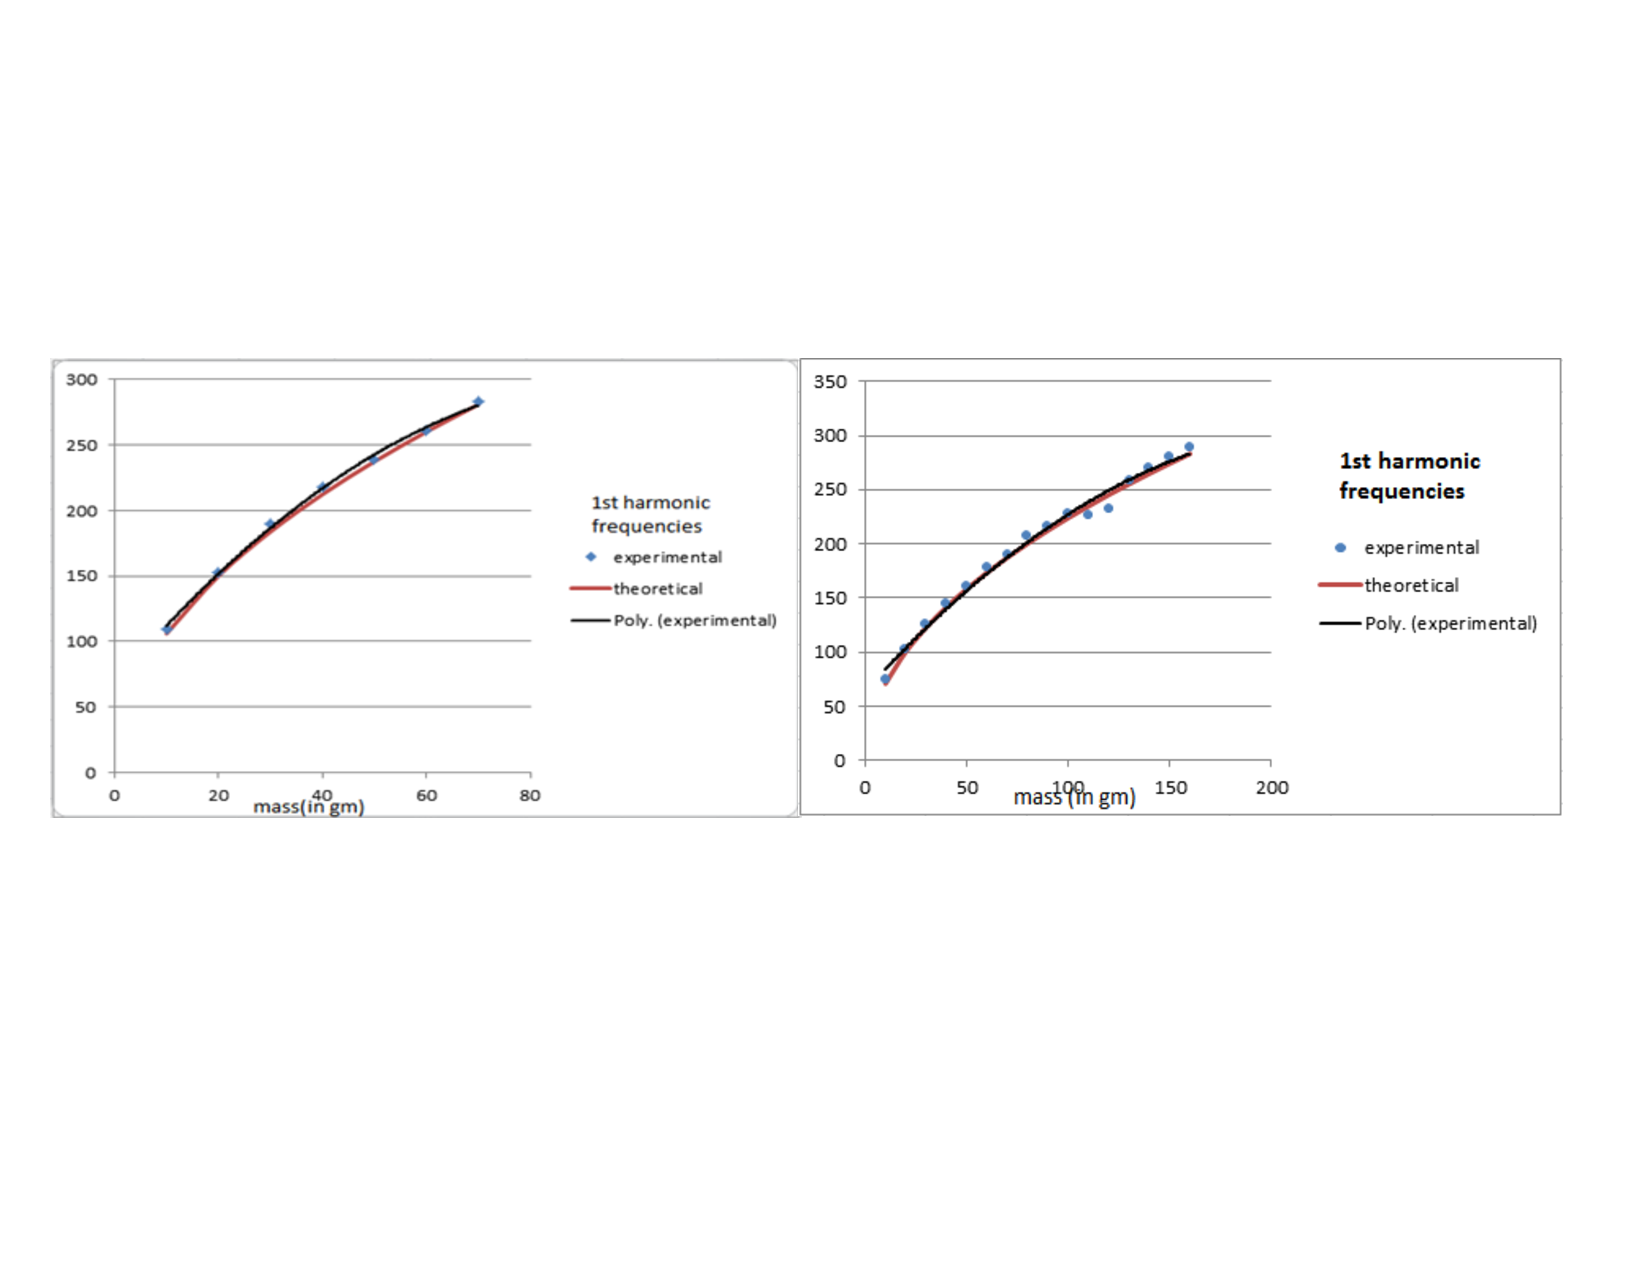
\includegraphics[width=1.0\textwidth]{STT_WireTensionTests}
\end{cdrfigure}


%\textbf{ \textit{Test Straw Chamber}} \\
A test chamber with 48 straws of the same dimensions as those for the FGT but
with 1-m length is available for use in operational studies aimed at understanding
the gas flow rates and for finalizing the preamplifier selection
parameters.  Figure~\ref{fig:STT_TestStrawChamber} shows the
operational pulse image with Ar+CO$_2$ (80:20) gas taken with cosmic
rays. The voltage versus amplitude for one of the straws is also shown
in Figure~\ref{fig:STT_TestStrawChamber} to establish the QA/QC
procedure for the fabricated straws.
\begin{cdrfigure}[Pulse and voltage-amplitude for the test straw chamber]
{STT_TestStrawChamber}{Example of pulse from the test straw chamber (left) and
measurement of voltage vs. amplitude for one of the straws in the test chamber (right).}
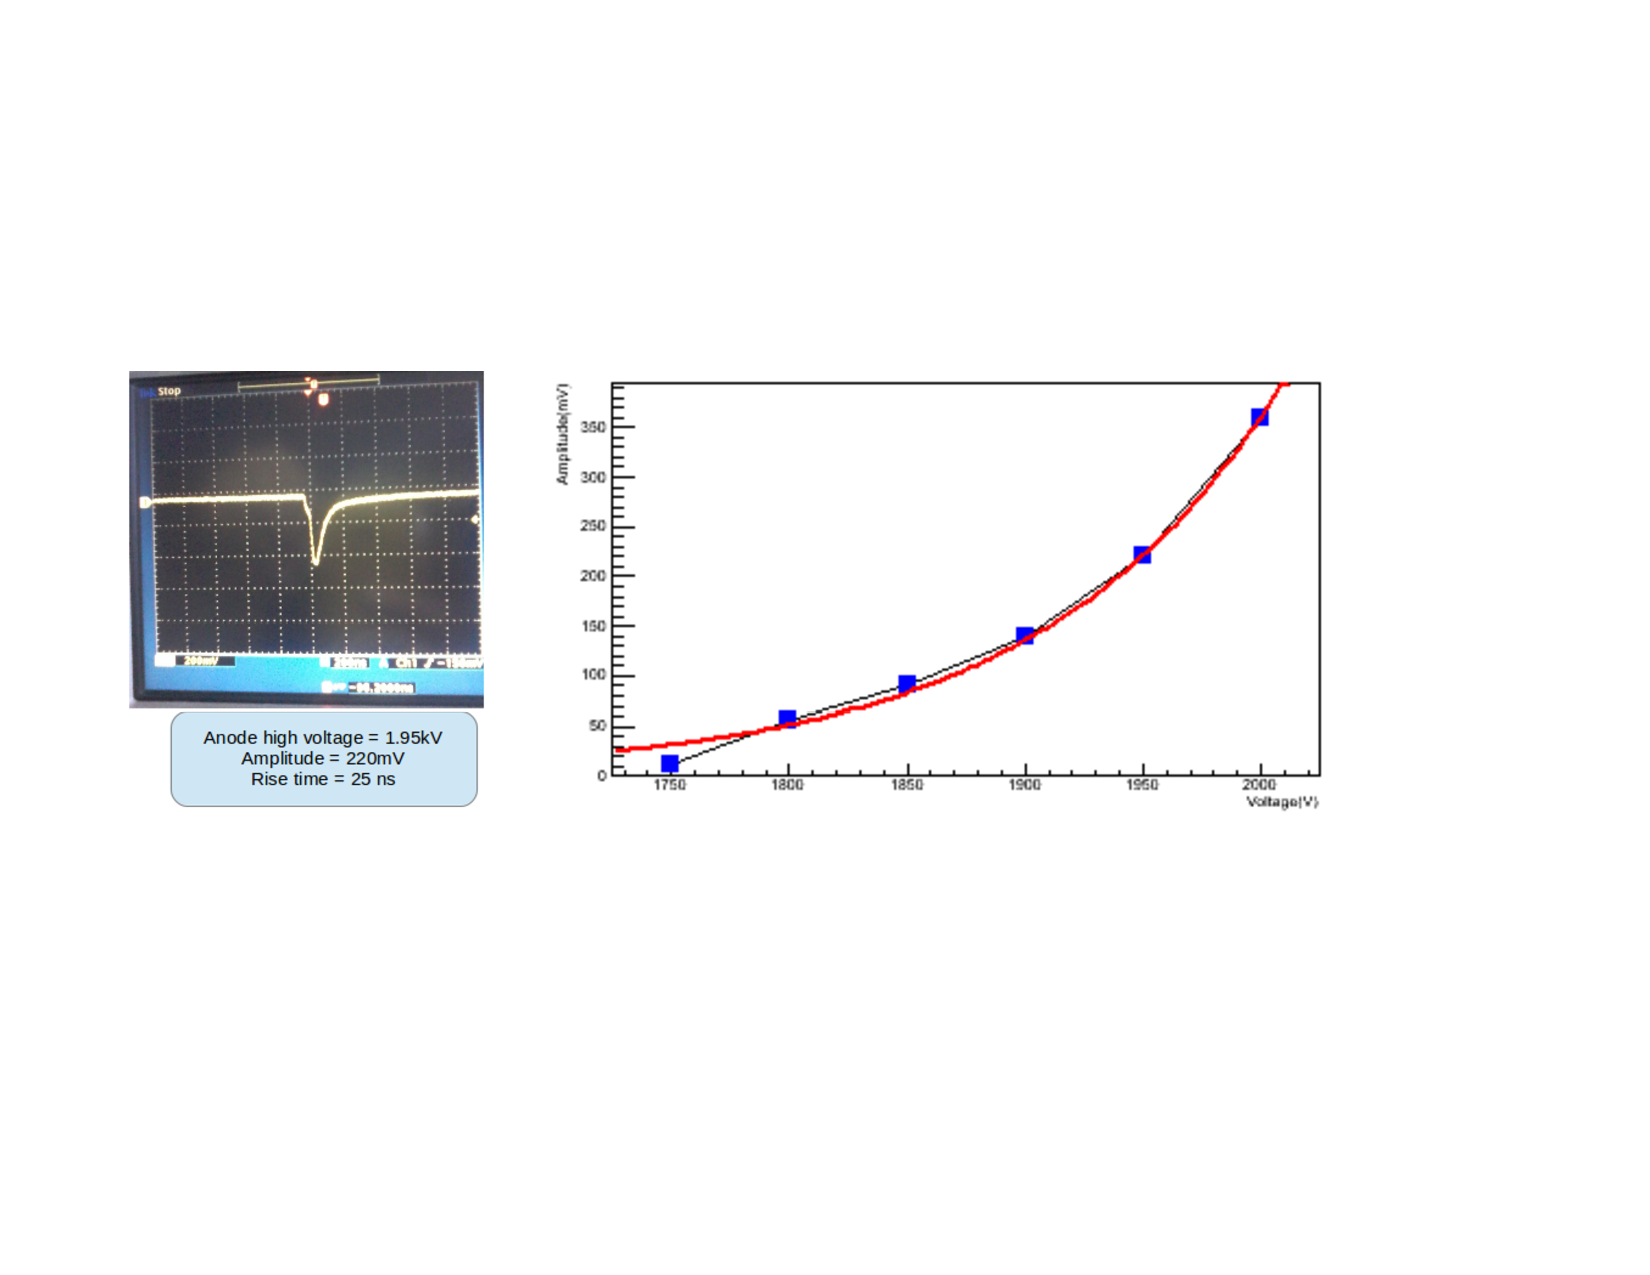
\includegraphics[width=1.0\textwidth]{STT_TestStrawChamber}
\end{cdrfigure}


%\textbf{ \textit{Front-end Electronics}} \\
We are performing some tests of prototype electronics for the signal readout. 
A four-channel preamplifier has been
tested with the test chamber using a radioactive source, and the signal
has been recorded as shown in Figure~\ref{fig:STT_SignalPreAmp}.  The
back-end DAQ is still being worked out and would follow the description 
in Section~\ref{cdrsec:detectors-nd-ref-fgt-instrum}. At
present both CAMAC- and VME-based DAQ are available. In addition, a $\mu$TCA-based fast
DAQ has also been setup. 
\begin{cdrfigure}[Signal from single straw using the BARC preamp and source]
{STT_SignalPreAmp}{Signal from single straw using the BARC (Bhabha Atomic Research Center) preamp and source.}
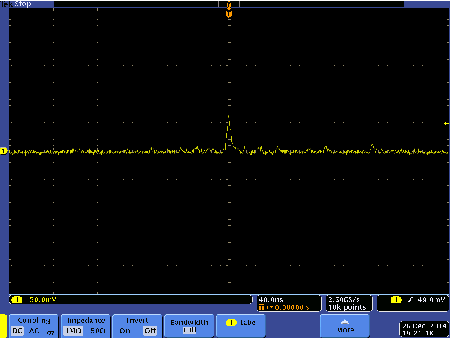
\includegraphics[width=0.6\textwidth]{STT_SignalPreAmp}
\end{cdrfigure}

%\textbf{ \textit{Other Activities}} \\
Other activities are in progress. As part of the prototyping, 50 straws of 1.8~m from Lamina
Dielectrics Ltd., in UK, and 1~km of 30~$\mu$m anode wire from Luma
Sweden has been procured. The Optical bench for the fabrication of the
straws has been setup.  Two pre-mixed gas bottles of Ar+CO$_2$ have been
procured. The operational gas mixture %being 
Xe+CO$_2$ will be added
soon. Local industry and vendors have been identified for the
manufacturing of nozzles, end-plugs, wire-spacers and steel
balls. Local workshops are available to fabricate the mechanical
structure to hold the straws in the prototype design and also to
fabricate a test stand for studies of efficiency and characteristics with
a radioactive source. Wire stringing, straw gluing and other tooling
setups are still to be established.


%\textbf{ \textit{Design of the Full-scale STT Modules}} \\
%We will optimize t
The final design of the STT modules will be optimized based on the
results obtained from the STT prototype and from all the related prototyping
activities listed above. This task includes a detailed FEM analysis to
assess the mechanical structure and the choice of the final
materials. The final design is intended to be ready for the
fabrication of the full-scale STT detector. 



\subsubsection{ECAL Detector}

In FGT the ECAL detector will occupy the space outside
the STT with $4\pi$ coverage.  The detailed description of this
detector is given in Section~\ref{cdrsec:detectors-nd-ref-fgt-ecal}.
The ECAL prototype will be a 2~m$\times$2~m module similar to the
downstream-ECAL design.  The half-scale downstream ECAL prototype
construction, which uses Pb as the absorber and extruded scintillator
with embedded fiber as the active detector system, will involve the
following steps:
\begin{itemize}
\item procure materials such as plastic scintillator bars, WLS fibers,
  SiPM, Pb sheets, etc.
\item set up mechanism to ensure the quality of the scintillator bars,
  fibers and Pb sheets
\item set up tools for the characterization of SiPMs
\item assemble scintillator bars in an Aluminum frame for a
  prototype layer formation
\item undertake R\&D for the coupling of the fiber to the SiPMs as well
  as the inserting of fiber in the scintillator
\item develop readout electronics for the prototype and set up a cosmic
  test stand with full DAQ
\item complete mechanical stability mechanism of the ECAL design 
\end{itemize}

The ECAL readout system is centered on a highly sensitive/high-gain SiPM. %The work to be undertaken
During the R\&D phase, SiPMs from Hamamatru, AdvanSiD and SiPM developed in India by SCL will be compared. 
Discussions have been started with all the vendors.

%\begin{itemize}
%\item comparison of SiPMs from Hamamatru, AdvanSiD and SiPM developed in India by SCL
%\item discussions are already on with all the vendors
%\end{itemize}

For optimizing the ECAL detector geometry, %an effort for 
GEANT4
simulations of the ECAL have already been initiated. The geometry in
the current GEANT4 simulation includes 58 layers of alternating
horizontal and vertical scintillator layers per 1.75~mm Pb along the
$z$-direction. In
the present configuration each scintillator layer is made of plastic scintillator
bars of dimensions 4~m$\times$2.5~cm$\times$1~cm, resulting in 160
bars per layer, and \num{9280} scintillator bars for the downstream ECAL .  
Figure~\ref{fig:ECAL_SimulationG4} shows
the longitudinal view of the electromagnetic shower in the downstream
ECAL by 2~GeV photons. Figure~\ref{fig:ECAL_detail} shows the design
of the Pb-scintillator assembly configuration for the ECAL.
\begin{cdrfigure}[Longitudinal view of the EM shower in
the downstream ECAL by 2 GeV photons]
{ECAL_SimulationG4}{Longitudinal view of the electromagnetic shower in
the downstream ECAL by 2 GeV photons.}
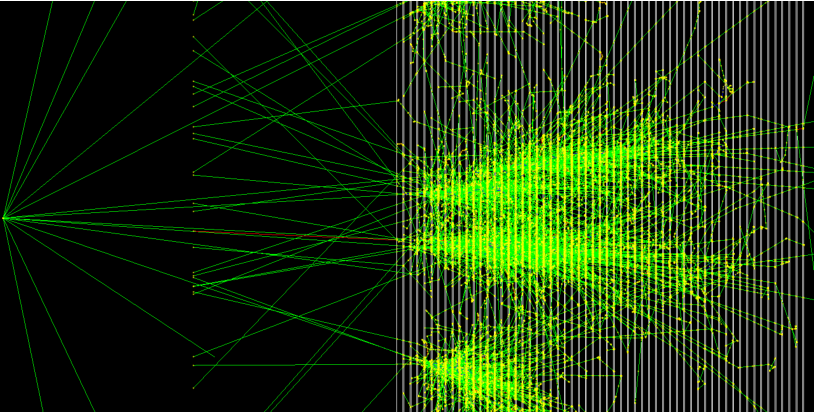
\includegraphics[width=0.6\textwidth]{ECAL_SimulationG4}
\end{cdrfigure}

For the construction of the prototype and for the assembly of the 
actual detector a
space of dimension 32~m$\times$12~m has been
identified. Construction of a class 10,000 clean room covering a
laboratory space of 12~m$\times$12~m is under consideration. %currently. 
Figure~\ref{fig:ECAL_LabIITG} shows the schematic diagram
of the laboratory refurbishment plan for the ECAL R\&D and fabrication
work.
\begin{cdrfigure}[Laboratory refurbishment plan for ECAL R\&D and assembly]
{ECAL_LabIITG}{Laboratory refurbishment plan for the ECAL R\&D and assembly work.}
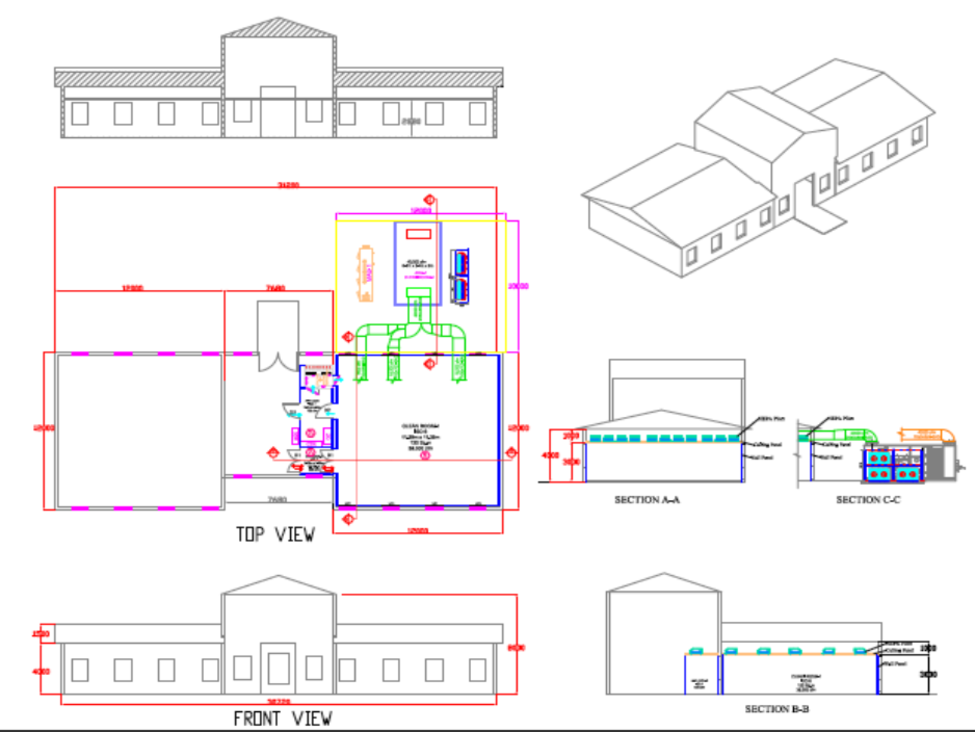
\includegraphics[width=0.6\textwidth]{ECAL_LabIITG}
\end{cdrfigure}


\subsubsection{Dipole Magnet Development}

The massive dipole magnet (Section~\ref{cdrsec:detectors-nd-ref-fgt-magnet}) for the FGT will
play a critical role since it will allow the particle-momentum measurements, will 
provide space for the MuID--RPC installations in the magnet steel, 
and will give structural support to the FGT. 
The planned magnet prototype
%envisaged prototype of the dipole magnet 
includes the engineering development of the tooling and
infrastructure. 
 % The, thus developed, infra-setup 
that will be used to produce one C out of the total 8 Cs of the
8.0-m long dipole.  The same C will be utilized in the final magnet
assembly. In a similar way, one of the four coils %would 
will be assembled
 to establish the procedure of coil winding and to measure the
operating characteristics.  Field simulation work is already at a very
advanced stage (see Figure~\ref{fig:Magnet_Bfield}) and the mechanical
designs are being produced.  (Steel dimensions are being optimized to house the muon
identification detectors.) Since it will be a
closed system, access to the inner detector systems is under extensive
study. % now.


\subsubsection{MuID--RPC Detector}

Muon identification will done with the Resistive Plate Chamber (RPC)
detectors made up of Bakelite electrodes.  The mounting structure for these
RPCs will be provided by the magnet steel (on sides and ends). %There has been an e
Extensive R\&D has already been done for such detectors and 
is being applied 
%the experience gained so far is being extended 
to the prototyping of the
muon identifiers. The size of the RPCs in FGT make it 
challenging to procure the raw material from industry, however an Indian 
industry has already been identified and a large 2.4-m$\times$1.2~m
RPC prototype has been assembled (see
Section~\ref{cdrsec:detectors-nd-ref-fgt-muonid}). The I-V
characteristics obtained for these RPCs are very encouraging. More such
RPCs will be fabricated during the prototyping phase and will be  
tested for sustained efficiency %over a period of time 
with variation
in ambient parameters, as the Bakelite is sensitive to such
changes. Some of the measured quantities are shown in
Figure~\ref{fig:RPC_PrototypeTests}.  The readout electronics is being
developed with input from similar R\&D done for the INO-ICAL
detector~\cite{1748-0221-7-10-P10003}. The gases standardly used in the RPC operations would need
substitution/replacement with more safe gases, due to the safety requirements for underground operation. 
An initiative in
this direction will be taken up during the prototyping phase.
\begin{cdrfigure}[RPC characteristics measured during the prototype development]
{RPC_PrototypeTests}{RPC characteristics measured during the prototype development.}
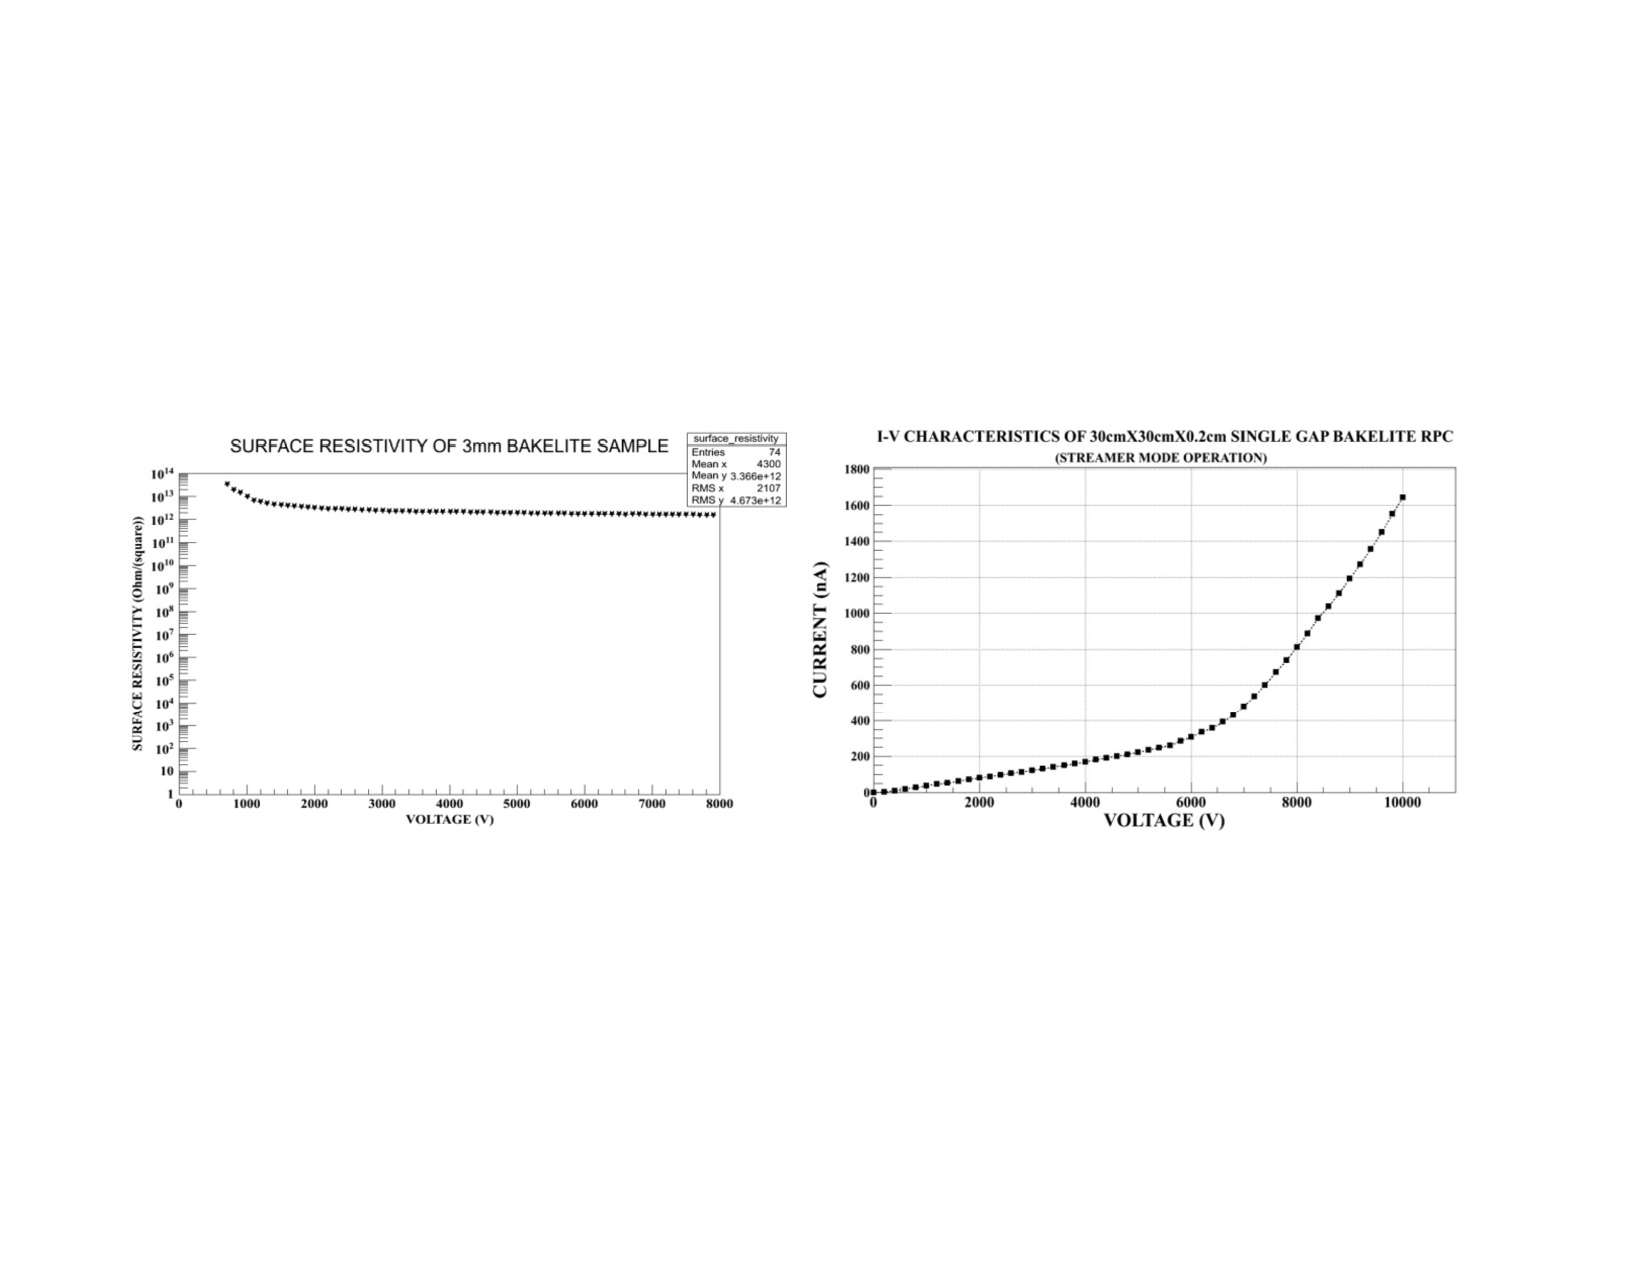
\includegraphics[width=1.0\textwidth]{RPC_PrototypeTests}
\end{cdrfigure}



\subsection{Beamline Measurement Detectors Prototyping Plan}
\label{sec:proto-nd-blm}
This Section describes recent and ongoing prototyping efforts for the detectors described in Section~\ref{sec:detectors-nd-ref-blm}.


\subsubsection{Prototype Development for the Cherenkov and Ionization Detectors}
\label{subsec:proto-blm-muon-cherenkov-proto}

A prototype Cherenkov counter, along with associated fully automated
gas systems, HV systems, and data acquisition system has been
constructed and is undergoing testing in the NuMI neutrino beam's Muon
Alcove 2. In addition, three diamond detectors~\cite{ref:CERNdiamond} (from CERN)
for ionization measurements have also been installed into the alcove. 
Figure~\ref{fig:Alcove2Cherenkov} shows the prototype detectors in
NuMI Alcove 2.
\begin{cdrfigure}[Muon gas Cherenkov counter]{Alcove2Cherenkov}
{A prototype muon gas Cherenkov detector for DUNE.
Muons travel through an L-shaped 4-inch Conflat pipe filled with a
pressurized gas. A flat mirror mirrors directs the optical photons
to a photo multiplier. The lower right inset shows the 20~bar MKS
pressure reading achieved by the Cherenkov gas system, and the inset
on the upper right shows the CERN/Cividec diamond detectors mounted to the Cherenkov housing.}
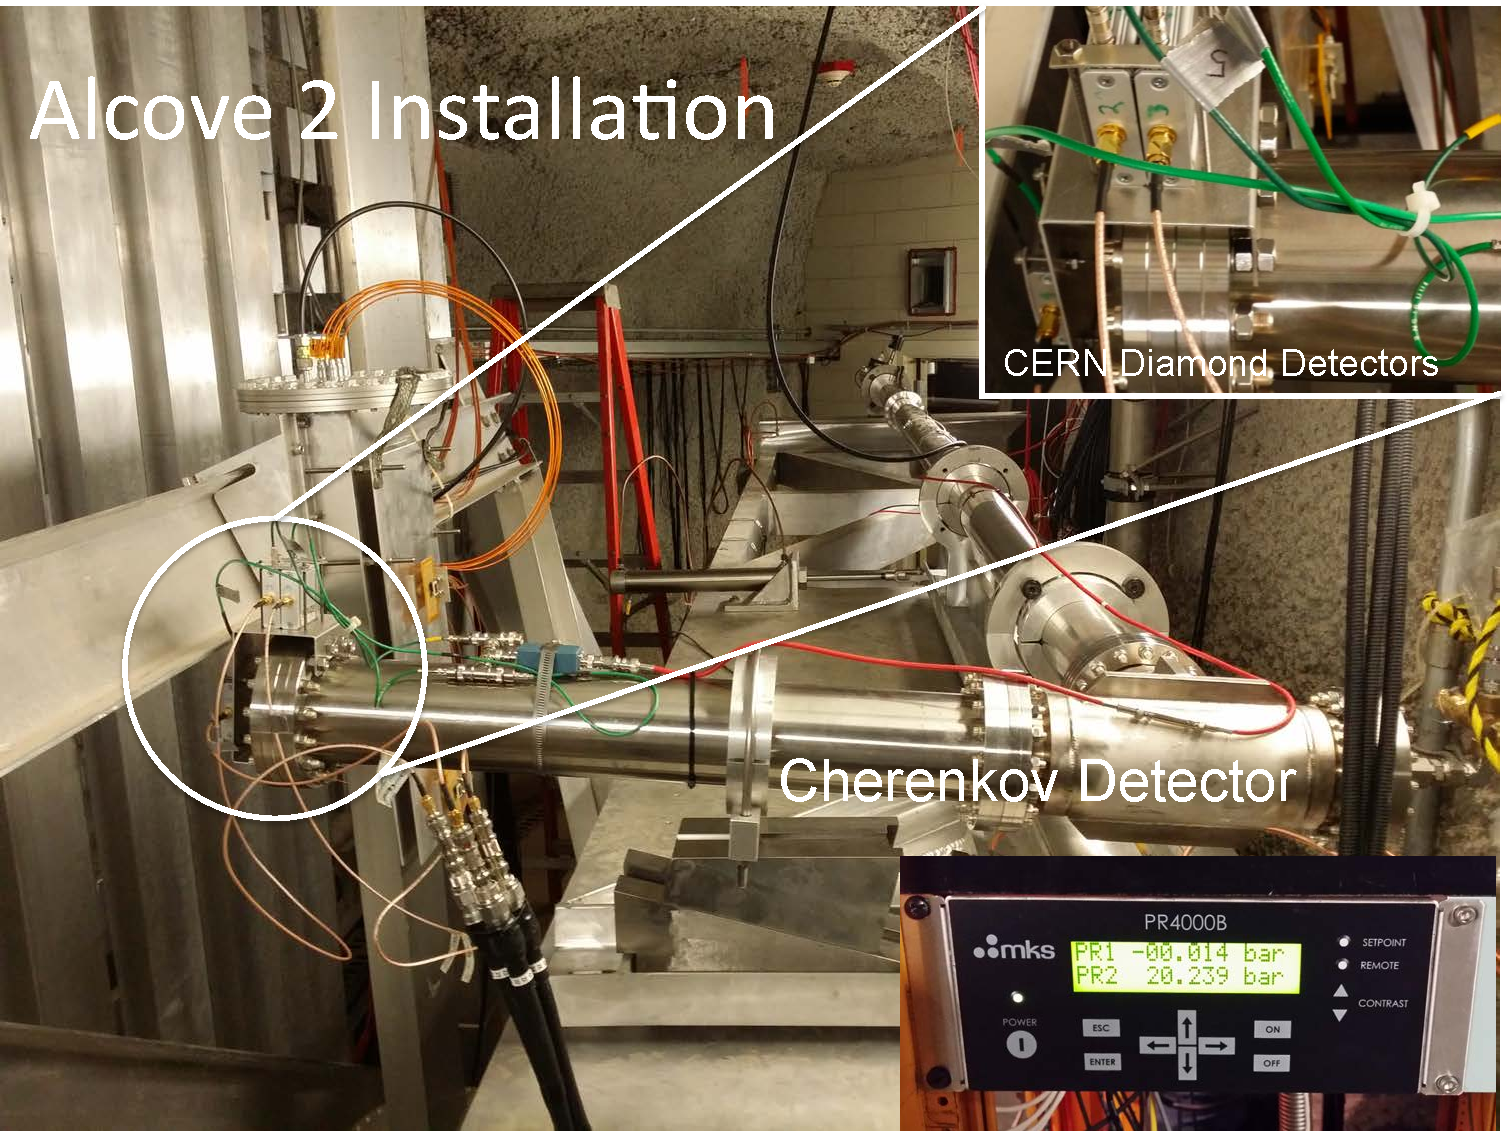
\includegraphics[width=6.in]{Alcove2Cherenkov}
\end{cdrfigure}

The counter has an automated gas system with an adjustable % settable 
pressure that
ranges from vacuum to 20~atm, corresponding to muon Cherenkov
thresholds of 200~GeV/c and 1~GeV/c, respectively. When operated at
vacuum, a photomultiplier tube (PMT) registers all background light unrelated to the gas,
e.g., transition radiation and light from particles hitting the window and
PMT glass.  These contributions are observed to be very small relative
to the coherent, directional Cherenkov light.

The counter is constructed with a 1-m long radiator section as shown
in Figure~\ref{fig:CherenkovCounterDetail} . A 20-foot extension
allows the reflected Cherenkov light to travel to a sapphire pressure
window viewed by a PMT.
\begin{cdrfigure}[Muon gas Cherenkov counter detail]{CherenkovCounterDetail}
{A prototype muon gas Cherenkov detector for DUNE.  }
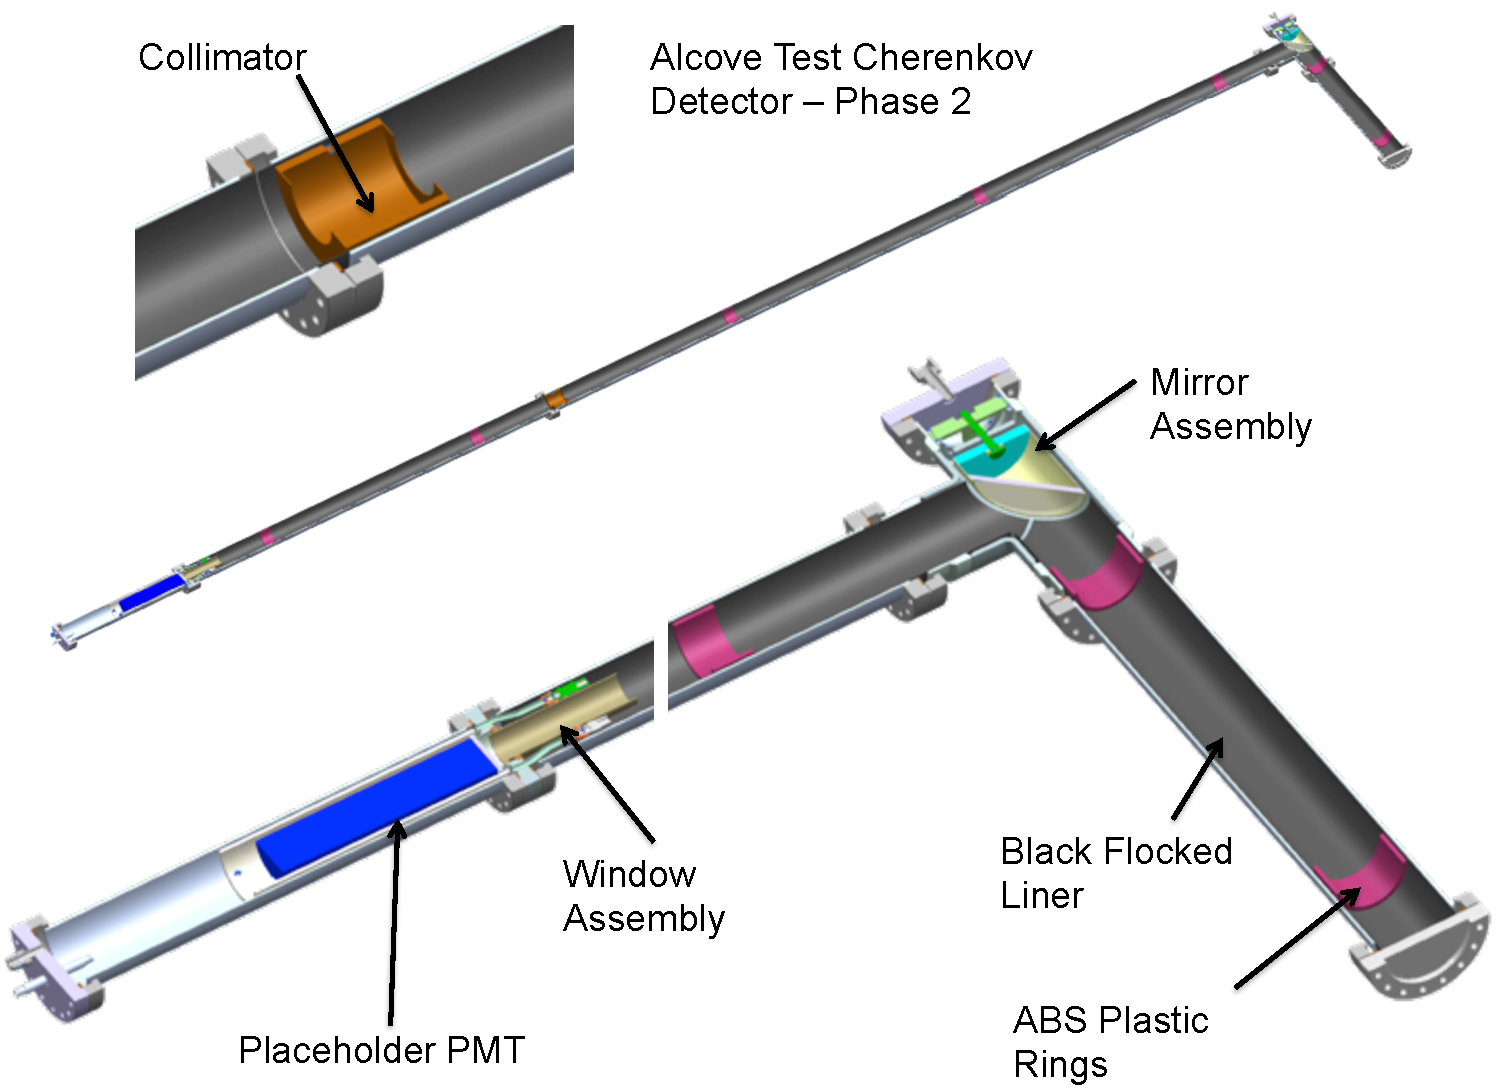
\includegraphics[width=6.in]{CherenkovCounterDetail.pdf}
\end{cdrfigure}


The prototype has been %is now 
fully integrated into NuMI operations and
real-time waveforms can be viewed online as shown in
Figure~\ref{fig:MuonDetectorWaveforms}.
\begin{cdrfigure}[Muon detector waveforms]{MuonDetectorWaveforms}
{The real-time display of the muon detector prototypes in operation
on the NuMI beam line. The top two panels are the Cherenkov counter
and CERN diamond detector. The signals are
transmitted through low-loss heliax cable, then the waveform
is digitized at 2.5~GHz with a 12-bit dynamic range, and is
recorded onto disk storage for analysis. The signal from the
muons is contained in the short beam pulse ``buckets'' created
by the accelerator RF structure. The fast timing allows the
prompt muon signal to be easily separated from potential backgrounds
such as stopped-muon decays, beta decays, and neutrons.}
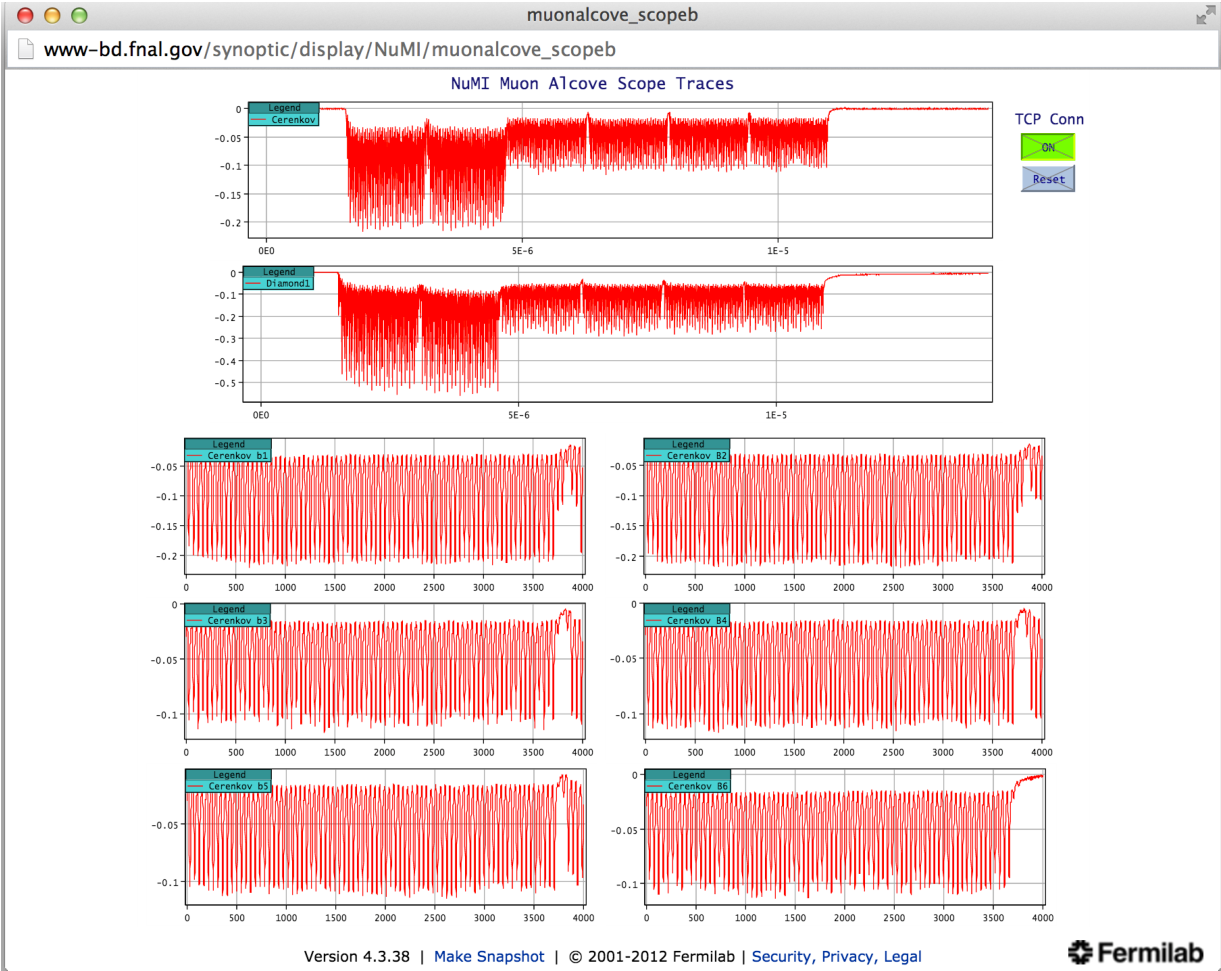
\includegraphics[width=5in]{MuonDetectorWaveforms}
\end{cdrfigure}
The top panel shows the waveform from the Cherenkov counter at 2~atm
gas pressure, which corresponds to a muon momentum threshold of
3~GeV/c. The second panel shows the waveform from a 9~mm$\times$9~mm
diamond detector mounted to the front flange of the Cherenkov radiator
section, as shown in the inset of Figure~\ref{fig:Alcove2Cherenkov}.

The extracted NuMI proton beam produces a signal in the  Resistive Wall 
Monitor (RWM) that is also recorded with an identical digitizer.  This allows a direct,
bucket-by-bucket (individual proton pulses) comparison of the proton
current onto the NuMI primary proton target, and the muons are measured
after the absorber with a 400-ps time resolution.

\subsubsection{Prototype Development of the Stopped-Muon Counters}

Prototype development activity for the Michel-electron detectors will
be divided into studies of (1) the rate of particles and the radiation environment where
the detectors will be located, and (2) development of the counters
themselves.

The radiation environment will be studied both with Monte Carlo
simulations and by measurements from initial prototype detectors
in the NuMI muon alcoves~\cite{ref:NuMIBeamMonitors}.
The prototypes will be installed into the alcoves in 2016 and 2017.
Studies will be performed to determine if the photon sensors
can survive the radiation environment at the location of the Michel
detector. If the sensors can survive, they can be attached directly to
the Cherenkov medium; if not, optical guides will have to bring the
light to a lower-radiation area, to the side of the beam. Potential
radiation damage to the Cherenkov radiator itself will also be
studied.

The detector design will focus on selecting radiator and shielding
material, photon-detection technology and control/readout
hardware. Possible radiators include ones that use aerogel (these may be designed to
be replaced periodically) and ones that use flowing liquids such as H$_2$O or
mineral oil. Long-timescale saturation from the very high-rate
environment of the beam spill could affect the photon-counting
devices~\cite{ref:HighRateCounting}. Thus, it will likely be necessary
to design fast-switching, high-voltage circuits that turn on the
photon counters in the first few microseconds after the spill is
over. A similar system was developed in the 1990s for the Brookhaven
Muon (g-2) Experiment~\cite{ref:G2} .

%\textbf{ \textit{Current Prototyping Activities}} \\
A second set of muon detectors, the final 
%\fixme{really want to say `final'?i - yes} 
DUNE design, are being
constructed at this time (2015). They are being installed directly
behind the NuMI proton beam dump (Muon Alcove 1), mounted on a movable stand which has undergone an engineering
review at Fermilab. 
%
The entire setup, detectors and stand, will be
suitable for use in the DUNE beam. The higher-radiation environment of Alcove 1 is more representative %similar 
than Alcove 2 of the conditions in the eventual DUNE installation, and will 
allow a more accurate calibration in the NuMI
beam. The setup will be eventually transferred the DUNE Absorber Hall. 